\documentclass[10pt]{article}

\usepackage{amsmath}
\usepackage{enumitem}
\usepackage{xcolor}
\usepackage{pgfplots}
\usepackage{tikz}
\usepackage{cleveref}

% Define bar chart colors
%
\definecolor{bblue}{HTML}{4F81BD}
\definecolor{rred}{HTML}{C0504D}
\definecolor{ggreen}{HTML}{9BBB59}
\definecolor{ppurple}{HTML}{9F4C7C}
\definecolor{oorange}{HTML}{FFA500}
\definecolor{yyellow}{HTML}{44DDDD}

\usepackage{titlesec}
\titlespacing*{\section}{0pt}{0.4\baselineskip}{0.2\baselineskip}
\setlist[enumerate]{itemsep=0mm}

% MARGINS (DO NOT EDIT) ---------------------------------------------
\oddsidemargin  0in \evensidemargin 0in \topmargin 0in
\headheight 0in \headsep 0.1in
\textwidth  6.5in \textheight 9.0in
\parskip 1.25ex  \parindent 0ex \footskip 20pt
% ---------------------------------------------------------------------------------

\title{Application of Machine Learning to Link Prediction}
\author{Kyle Julian (kjulian3), Wayne Lu (waynelu)}
\date{December 16, 2016}
\begin{document}
\maketitle
   
\section{Introduction}
Real-world networks evolve over time as new nodes and links are added. Link prediction algorithms use historical data in order to predict the appearance of a new links in the network or to identify links which may exist but are not represented in the data. The application of link prediction is most commonly seen in recommendation engines, such as new connections on social networks or related products on shopping sites. Traditional approaches involve the calculation of a heuristic similarity score for a pair of nodes, such as the number of common neighbors or the shortest path length connecting the nodes, where pairs of nodes with the highest similarity scores are considered the most likely edges.

In this project, we will apply supervised learning algorithms to the link prediction prediction problem using a large set of topological features. Given a network at two different points in time, we train a learning algorithm to identify pairs of edges which appear in the newer network but not in the older network. Then, for a pair of nodes, we use the classification probability of the learning algorithm as our link prediction heuristic. Furthermore, we show that our network-specific heuristics outperform generic heuristics such as the Adamic/Adar coefficient and the Jaccard coefficient.

\section{Related Work}
Link prediction and the application of machine learning techniques to link prediction both have significant corpuses of work behind them. Adamic and Adar used similarities between the web pages of students at MIT and Stanford to predict friendship. Notably, in generating a similarity score, common features between students were weighted by the inverse log of their overall frequency [1]. Liben-Nowell and Kleinberg applied to idea of link predictors to network evolution by evaluating how well link prediction heuristics can account for the growth of a network over time. They used a variety of topological heuristic scores as link predictors for arXiv co-authorship networks and compared their relative performances [2]. In the same vein, Zhou et al. evaluated the performance of local similarity heuristics on six real-world networks from different domains and then described a new local similarity measure based on resource distribution through common neighbors [3].

Al Hasan et al. applied supervised learning to link prediction on the BIOBASE and DBPL co-authorship networks, using both topological and domain-specific proximity features [4]. Leskovec et al. applied supervised learning to edge sign detection in real-world social networks, notably comparing the performance of trained algorithms across different datasets and applying partial triads as features to capture the relationship of two nodes through their neighbors [5].

\section{Datasets and Features}
The datasets used in this project are publicly available from the Stanford Network Analysis Project (SNAP) [6]. Our datasets consist of the Wikipedia Request for Adminship (RfA) voting network, five arXiv co-authorship networks, and two snapshots of the Slashdot Zoo social network. For each dataset graph $G = (V, E)$, examples were generating via the following process:
\begin{enumerate}
\item Remove low-degree nodes from $G$ ($d_{\min} = 5$ for Slashdot graphs, $d_{\min} = 3$ for all others) to induce a subgraph $G_{n} = (V', E')$
\item Let $E''$ be a random sample of 10\% of the edges of $E'$. Let $G_{o} = (V', E' - E'')$
\item Let $P \subset V' \times V'$ be all pairs of nodes $(u, v)$ such that $u$ and $v$ share a common neighbor, but $(u, v) \not \in E'$ and $u \neq v$
\item Apply a 70-30 training-testing split to $E''$ and $P$ and extract the topological features using $G_{o}$.
\end{enumerate}

\begin{table}[h]
	\centering
   		\begin{tabular}{l|r|r|r|r}
                	\textbf{Dataset} & \textbf{Nodes} & \textbf{Edges} & \textbf{Training} & \textbf{Testing} \\ \hline
                	wiki-Vote & 3772 & 98978 & 28491 & 66479 \\ \hline
                	ca-AstroPh & 14175 & 189929 & 56976 & 132944\\ \hline
                	ca-CondMat & 14645 & 78785 & 23634 & 55146 \\ \hline
                	ca-GrQc & 2155 & 9967 & 2988 & 6972 \\ \hline
                	ca-HepPh & 7225 & 110243 & 33072 & 77168 \\ \hline
                	ca-HepTh & 4306 & 17306 & 5190 & 12110 \\ \hline
		slashdot0811 & 77360 & 905468 & 271638 & 633822 \\ \hline
		slashdot0902 & 82168 & 948464 & 284538 & 663922 \\
                	\end{tabular}
	\caption{Summary statistics of the pruned datasets}
\end{table}

The removal of a random sample of edges simulates the state of the graph at a previous point in time, $G_{o}$. Our positive training examples then consist of edges which do not appear in $G_o$ but do appear in $G_n$, simulating the growth of the network. We balance our positive examples with negative examples which consist of pairs of nodes which do not form an edge in $G_n$. We then extract features from $G_o$ because our goal to train a learner to predict edges in $G_n$ using the current state of $G_o$.

For a pair of nodes $(u, v)$, we extract the three different classes of features. There are eight degree features which are $d_{\text{in}}(u)$, $d_{\text{out}}(u)$, $d_{\text{in}}(u) / d_{\text{out}}(u)$, $d_{\text{out}}(u) / d_{\text{in}}(u)$, $d_{\text{in}}(v)$, $d_{\text{out}}(v)$, $d_{\text{in}}(v) / d_{\text{out}}(v)$, and $d_{\text{out}}(v) / d_{\text{in}}(v)$. There are eight triad features which are defined by the number of partial triads that $u, v$ form with a common neighbor $w$. There are four types of triads with participation frequency for each denoted as $t_1$, $t_2$, $t_3$, and $t_4$. The eight triad features are: $t_1$, $t_2$, $t_3$, $t_4$, $t_1 / C(u, v)$, $t_2 / C(u, v)$, $t_3 /  C(u, v)$, and $t_4 / C(u, v)$, where $C(u, v)$ is the total number of common neighbors. Finally, there are four heuristic features: common neighbors ($\Gamma(u) \cap \Gamma(v)$), the Adamic/Adar coefficient ($\sum_{w \in \Gamma(u) \cap \Gamma(v)} \frac{1}{\log |\Gamma(w)|}$), the Jaccard coefficient ($\frac{|\Gamma(u) \cap \Gamma(v)|}{|\Gamma(u) \cup \Gamma(v)|}$), and the preferential attachment coefficient ($|\Gamma(u)| \cdot |\Gamma(v)|$).

\begin{table}[h]
        \centering
            \begin{tabular}{c|c|c|c}
            $u \rightarrow w \rightarrow v$ & $u \rightarrow w \leftarrow v$ & $u \leftarrow w \rightarrow v$ & $u \leftarrow w \leftarrow v$ \\
            $t_1$ & $t_2$ & $t_3$ & $t_4$
            \end{tabular}
          \caption{The four triad types that $u$ and $v$ can form with a common neighbor $w$}
\end{table}

\section{Methods}
We tested three different supervised learning algorithms for link prediction. The first algorithm, logistic regression, seeks to find $\theta$ to maximize
\begin{equation}
h_\theta (x) = \frac{1}{1+e^{-\theta^Tx}}
\end{equation}
This learner uses the logistic function, $g(z) = \frac{1}{1+\exp{-z}}$, which maps $\theta^T x$ to values between 0 and 1. Since we are training a binary classifier, the hypothesis represents the probability that the training label, $y$, is true. Using stochastic gradient ascent with the update rule,
\begin{equation}
\theta_j := \theta_j + \alpha (y^{(i)}-h_\theta (x^{(i)})x_j^{(i)}
\end{equation}
we can iteratively update $\theta$ to maximize the likelihood that the hypothesis is correct. Logistic regression is a standard algorithm for binary classification and serves as our baseline learner.

Our second learning algorithm is random forests which creates an ensemble of random trees and combines the individual decisions of the trees by taking the mode of the decisions. This algorithm draws random samples from the dataset with replacement and trains a decision tree on the sampled data. The decision tree is created by choosing splits that maximize the Gini impurity. The Gini impurity is a measure of disorder in a set by calculating the probability of mislabeling a random element in the set if it were labeled randomly. The split that decreases the Gini impurity the most is chosen as the decision split, and the tree is formed in a greedy fashion by sub-dividing the sets of training data into smaller and less disordered sets.

In many cases, decision trees can overfit to their training data too much. Some methods to improve this behavior include pruning the tree by stopping the decision splits where the Gini impurity falls below some threshold. The method chosen here to reduce over-fitting is to train multiple decision trees on random subsets of the data and combining the individual decisions into one decision. Each individual tree may ovefit to its random training data, but in general the forest of decision trees will be less biased to the draw samples. 

Our last supervised learning method trains a neural network to classify the edges. For a binomial classification network, the output of the network will have two outputs that go through a softmax activation function:
\begin{equation}
	h(z)_j = \frac{e^{z_j}}{e^{z_0}+e^{z_1}} \; j \in \{0,1\}
\end{equation}
The softmax converts the network outputs into a probability distribution in which the larger valued output will have a higher probability. The training labels can be represented as the true label probabilities, which take the form of one-hot vectors. We can compare the probability distributions using the cross-entropy method, which is a measure of difference between two probability distributions:
\begin{equation}
L(p,q) = -\sum_{x}p(x) \log q(x)
\end{equation}
We can use stochastic gradient descent with cross-entropy loss to iteratively update the network parameters to reduce the loss as much as possible. The result is a network that produces accurate probability estimates of the data labels.

\section{Results and Discussion}
We implemented the three learning algorithms in scikit-learn. The examples were not normalized because we wanted to create models that predict edges accurately even on datasets with different means and variances, and normalizing the datasets inhibits cross-prediction testing. To reduce over-fitting, the logistic regression and neural network use L2 regularization, which adds a penalty to the cost function for having larger weights. Logistic regression was optimized using limited-memory Broyden-Fletcher-Goldfarb-Shanno (LBFGS), an approximate quasi-Newton method [7]. The random forest generates 11 random trees and draws the same number of samples as are present in the data set, but uses replacement to create distributions that differ. The neural network has 5 hidden layers of 30 units each. Testing a few datasets with different network architectures showed that this shape gave the best performance without increasing the size of the network too much. Adam was used as the network optimizer, which estimates lower order moments of the loss in order to minimize loss very quickly without the need for finely tuning other parameters such as learning rate and momentum [8].

We trained each learner on three different subsets of the features to better understand their value in learning. The first subset consists of only the degree features. The second subset uses the degree and the triad features. The third subset consists of all features. As a baseline for the performance of our learners, we used the Adamic/Adar coefficient.

To compute test accuracies, we want to measure how accurately the learner outputs a similarity heuristic rather than its overall accuracy. So, given the test set for each dataset, which includes edges not in $G_o$ but present in $G_n$, we use the learner to predict the probabilities that each node pair contains a link. Let $k$ be the number of positive test examples. Then, our testing accuracy is the proportion of the $k$ most probable node pairs which are also positive examples, as shown in \Cref{fig_test}.

\begin{figure}[ht]
	\centering
	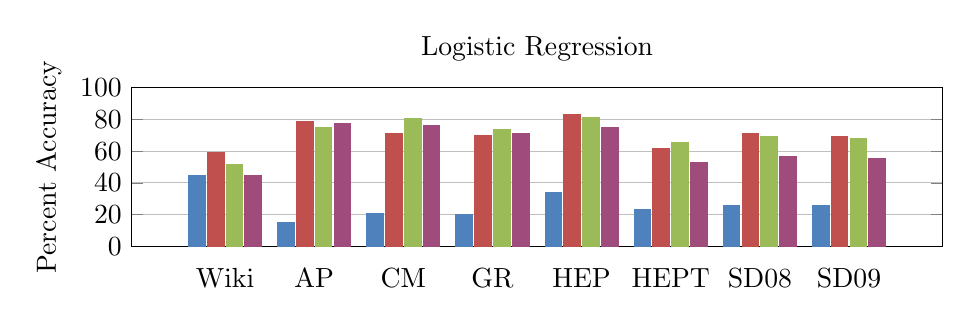
\begin{tikzpicture}
\begin{axis}[
width  = 0.98*\textwidth,
height = 3.6cm,
major x tick style = transparent,
ybar=2*\pgflinewidth,
bar width=6pt,
ymajorgrids = true,
ylabel = {Percent Accuracy},
%xlabel = {Data Set Used in Training},
symbolic x coords={Wiki,AP,CM,GR, HEP, HEPT,SD08,SD09},
xtick = data,
ytick = {0,20,40,60,80,100},
title = {Logistic Regression},
scaled y ticks = false,
enlarge x limits=0.15,
ymin=0,
ymax=100,
legend cell align=left,
legend style={
	at={(1.02,0)},
	anchor=south west,
	column sep=1ex
}
]
\addplot[style={bblue,fill=bblue,mark=none}]
coordinates {(Wiki, 44.47) (AP,15.31) (CM,20.58) (GR,20.13) (HEP,33.88) (HEPT, 23.17) (SD08, 25.79) (SD09, 26.00)};

\addplot[style={rred,fill=rred,mark=none}]
coordinates {(Wiki, 59.23) (AP,78.72) (CM,71.38) (GR,69.80) (HEP,82.88) (HEPT, 61.78) (SD08, 71.13) (SD09, 69.25)};

\addplot[style={ggreen,fill=ggreen,mark=none}]
coordinates {(Wiki, 51.55) (AP,74.61) (CM,80.44) (GR,73.83) (HEP,81.43) (HEPT, 65.25) (SD08, 69.40) (SD09, 68.18)};

\addplot[style={ppurple,fill=ppurple,mark=none}]
coordinates {(Wiki, 44.9) (AP,77.66) (CM,76.120) (GR,71.140) (HEP,74.95) (HEPT, 52.900) (SD08, 56.3) (SD09, 55.4)};

%legend{Basic Features, Basic and Triad, All Features, Adamic Heuristic}
\end{axis}
\end{tikzpicture}	
	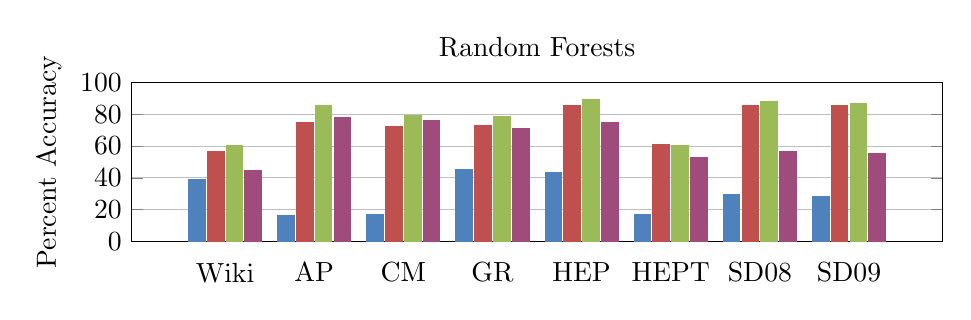
\begin{tikzpicture}
\begin{axis}[
	width  = 0.98*\textwidth,
	height = 3.6cm,
	major x tick style = transparent,
	ybar=2*\pgflinewidth,
	bar width=6pt,
	ymajorgrids = true,
	ylabel = {Percent Accuracy},
	%xlabel = {Data Set Used in Training},
	symbolic x coords={Wiki,AP,CM,GR, HEP, HEPT,SD08,SD09},
	xtick = data,
	ytick = {0,20,40,60,80,100},
	title = {Random Forests},
	scaled y ticks = false,
	enlarge x limits=0.15,
	ymin=0,
	ymax=100,
	legend cell align=left,
	legend style={
		at={(1.02,0)},
		anchor=south west,
		column sep=1ex
	}
]
	\addplot[style={bblue,fill=bblue,mark=none}]
	coordinates {(Wiki, 39.02) (AP,16.117) (CM,16.765) (GR,44.966) (HEP,43.436) (HEPT, 16.602) (SD08, 29.366) (SD09, 27.938)};
	
	\addplot[style={rred,fill=rred,mark=none}]
	coordinates {(Wiki, 56.469) (AP,74.51) (CM,72.142) (GR,73.154) (HEP,85.602) (HEPT, 61.004) (SD08, 85.798) (SD09, 85.300)};
	
	\addplot[style={ggreen,fill=ggreen,mark=none}]
	coordinates {(Wiki, 60.175) (AP,85.74) (CM,79.254) (GR,78.523) (HEP,88.990) (HEPT, 60.618) (SD08, 87.712) (SD09, 86.958)};
	
	\addplot[style={ppurple,fill=ppurple,mark=none}]
	coordinates {(Wiki, 44.900) (AP,77.66) (CM,76.120) (GR,71.140) (HEP,74.95) (HEPT, 52.900) (SD08, 56.3) (SD09, 55.4)};
	
	%\legend{Basic Features, Basic and Triad, All Features, Adamic Heuristic}
\end{axis}
\end{tikzpicture}	
	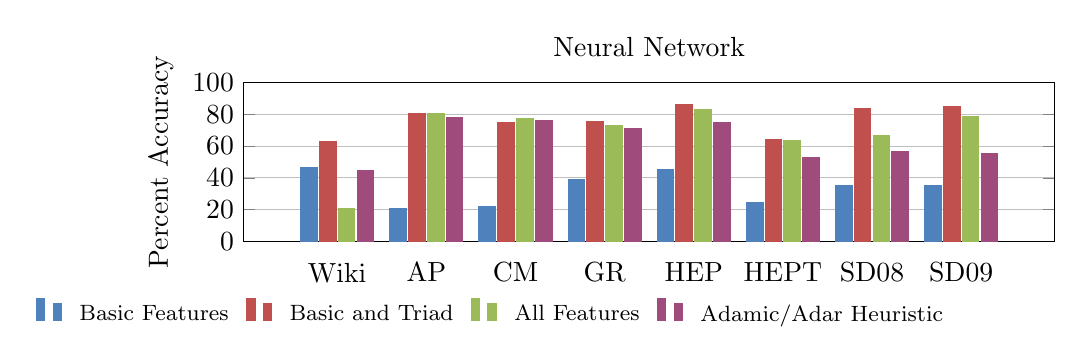
\begin{tikzpicture}
\begin{axis}[
	width  = 0.98*\textwidth,
	height = 3.6cm,
	major x tick style = transparent,
	ybar=2*\pgflinewidth,
	bar width=6pt,
	ymajorgrids = true,
	ylabel = {Percent Accuracy},
	%xlabel = {Data Set Used in Training},
	symbolic x coords={Wiki,AP,CM,GR, HEP, HEPT,SD08,SD09},
	xtick = data,
	ytick = {0,20,40,60,80,100},
	title = {Neural Network},
	scaled y ticks = false,
	enlarge x limits=0.15,
	ymin=0,
	ymax=100,
	%legend cell align=left,
	legend style={draw=none,legend columns=4,column sep=1ex,at={(0.88,-0.6)},anchor=south east,legend cell align=left,align=left,fill=white,font=\footnotesize}
	%legend style={
	%	at={(1.02,0)},
%		anchor=south west,
%		column sep=1ex
%	}
]
	\addplot[style={bblue,fill=bblue,mark=none}]
	coordinates {(Wiki, 46.77) (AP,20.61) (CM,21.76) (GR,38.93) (HEP,45.31) (HEPT, 24.71) (SD08, 35.41) (SD09, 35.30)};
	
	\addplot[style={rred,fill=rred,mark=none}]
	coordinates {(Wiki, 62.60) (AP,80.30) (CM,75.02) (GR,75.17) (HEP,86.03) (HEPT, 64.09) (SD08, 83.51) (SD09, 84.84)};
	
	\addplot[style={ggreen,fill=ggreen,mark=none}]
	coordinates {(Wiki, 20.55) (AP,80.44) (CM,77.39) (GR,73.15) (HEP,83.00) (HEPT, 63.32) (SD08, 66.93) (SD09, 78.53)};
	
	\addplot[style={ppurple,fill=ppurple,mark=none}]
	coordinates {(Wiki, 44.9) (AP,77.66) (CM,76.120) (GR,71.140) (HEP,74.95) (HEPT, 52.900) (SD08, 56.3) (SD09, 55.4)};
	
	\legend{Basic Features, Basic and Triad, All Features, Adamic/Adar Heuristic}
\end{axis}
\end{tikzpicture}	
	\label{fig_test}
	\caption{Accuracy of Link Predictions}
\end{figure}

The results show poor performance with only the basic features, which is expected given the features contain no information about the closeness of the two nodes. Including the triads, which has information about the proximity of the nodes, greatly improves the learners' performance and surpasses Adamic/Adar. Including the heuristic features helps random forests the most since the heuristics are made to function like a decision boundary, making them easy to integrate into the decision trees while the other learners to not benefit much from the heuristic features.

We also tested random forest models on each dataset to investigate cross-prediction performance. The results show that datasets test well on models trained on similar data sets, but the learners cannot generalize well for every graph. The features given vary drastically between the datasets, so feature values that may indicate a link in one graph may not be good indicators in a different graph. However, we can see strong correlation among the co-authorship graphs and the Slashdot datasets. This shows the learning algorithms can generalize well within a specific type of graph.
\begin{figure}[!ht]
	\centering
	\definecolor{yyyellow}{HTML}{DDDD44}
\definecolor{bblack}{HTML}{000000}
\definecolor{ccyan}{HTML}{44DDDD}

\begin{tikzpicture}
\begin{axis}[
	width  = 0.98*\textwidth,
	height = 3.6cm,
	major x tick style = transparent,
	ybar=2*\pgflinewidth,
	bar width=4pt,
	ymajorgrids = true,
	ylabel = {Percent Accuracy},
	%xlabel = {Data Set Used in Training},
	symbolic x coords={Wiki,AP,CM,GR, HEP, HEPT,SD08,SD09},
	xtick = data,
	ytick = {0,20,40,60,80,100},
	title = {Neural Network},
	scaled y ticks = false,
	enlarge x limits=0.15,
	ymin=0,
	ymax=100,
	%legend cell align=left,
	legend style={draw=none,legend columns=8,column sep=1ex,at={(0.88,-0.6)},anchor=south east,legend cell align=left,align=left,fill=white,font=\footnotesize}
	%legend style={
	%	at={(1.02,0)},
%		anchor=south west,
%		column sep=1ex
%	}
]
	\addplot[style={bblue,fill=bblue,mark=none}]
	coordinates {(Wiki, 57.75) (AP,8.01) (CM,15.97) (GR,16.04) (HEP,13.27) (HEPT, 20.96) (SD08, 38.95) (SD09, 43.33)};
	
	\addplot[style={rred,fill=rred,mark=none}]
	coordinates {(Wiki, 69.70) (AP,85.92) (CM,82.27) (GR,63.83) (HEP,81.04) (HEPT, 74.47) (SD08, 72.82) (SD09, 81.46)};
	
	\addplot[style={ggreen,fill=ggreen,mark=none}]
	coordinates {(Wiki, 64.86) (AP,78.32) (CM,79.76) (GR,73.2) (HEP,76.12) (HEPT, 71.21) (SD08, 69.60) (SD09, 72.73)};
	
	\addplot[style={ppurple,fill=ppurple,mark=none}]
	coordinates {(Wiki, 22.82) (AP,79.87) (CM,77.18) (GR,79.19) (HEP,75.17) (HEPT, 75.84) (SD08, 53.02) (SD09, 53.02)};
	
	
	\addplot[style={oorange,fill=oorange,mark=none}]
	coordinates {(Wiki, 68.06) (AP,85.06) (CM,67.27) (GR,79.37) (HEP,88.51) (HEPT, 47.01) (SD08, 82.21) (SD09, 80.82)};
	
	\addplot[style={yyyellow,fill=yyyellow,mark=none}]
	coordinates {(Wiki, 38.61) (AP,61.78) (CM,64.09) (GR,60.62) (HEP,58.69) (HEPT, 62.55) (SD08, 55.60) (SD09, 62.55)};
	
	\addplot[style={bblack,fill=bblack,mark=none}]
	coordinates {(Wiki, 26.69) (AP,29.9) (CM,30.6) (GR,28.4) (HEP,23.3) (HEPT, 18.9) (SD08, 88.28) (SD09, 87.48)};
	
	\addplot[style={ccyan,fill=ccyan,mark=none}]
	coordinates {(Wiki, 31.4) (AP,25.7) (CM,26.1) (GR,19.4) (HEP,19.3) (HEPT, 22.5) (SD08, 86.2) (SD09, 87.8)};
	
	
	
	\legend{Wiki,AP,CM,GR, HEP, HEPT,SD08,SD09}
\end{axis}
\end{tikzpicture}	
	\label{fig_cross}
	\caption{Accuracy of Cross Predictions}
\end{figure}


\section{Conclusion and Future Work}
Through supervised learning, we are able to train learning algorithms to calculate network-specific similarity scores which outperform traditional similarity heuristics. Notably, the use of only degree and triad features is enough to have higher accuracy than our baseline of the Adamic/Adar coefficient. Because our features depend on the topological structure of the network and do not use domain-specific features, it is possible to investigate similarities between network structures by cross-evaluating the performance of the learning algorithms.

It should be noted that our work roughly simulated network growth by randomly removing edges. Unfortunately, organic real-world network growth is not random but tends to follow a preferential attachment model. Therefore, to truly draw any conclusions, our methods should be used on real network growth data by capturing a network at two distinct times. Further evaluation of the generalizability of our methods across different domains is also warranted. In our results, we were able to show that networks drawn from different domains exhibited different network structures which degraded the performance of link predictors. However, we did not have the time to collect and process additional datasets to find networks from different domains which showed similar cross-performance.

\section{References}
\begin{enumerate}
\item Adamic, Lada A., and Eytan Adar. "Friends and neighbors on the web." \textit{Social networks} 25.3 (2003): 211-230.
\item Liben-Nowell, David, and Jon Kleinberg. "The link-prediction problem for social networks." \textit{Journal of the American society for information science and technology} 58.7 (2007): 1019-1031.
\item Zhou, Tao, Linyuan L�, and Yi-Cheng Zhang. "Predicting missing links via local information." \textit{The European Physical Journal} B 71.4 (2009): 623-630.
\item Al Hasan, Mohammad, et al. "Link prediction using supervised learning." \textit{SDM06: workshop on link analysis, counter-terrorism and security}. 2006.
\item Leskovec, Jure, Daniel Huttenlocher, and Jon Kleinberg. "Predicting positive and negative links in online social networks." \textit{Proceedings of the 19th international conference on World wide web. ACM}, 2010.
\item Leskovec, Jure and Andrej Krevl. "SNAP Datasets: Stanford Large Network Dataset Collection." http://snap.stanford.edu/data. Accessed December 2016.
\item Zhu, Ciyou, et al. "Algorithm 778: L-BFGS-B: Fortran subroutines for large-scale bound-constrained optimization." \textit{ACM Transactions on Mathematical Software (TOMS)} 23.4 (1997): 550-560.
\item Kingma, Diederik, and Jimmy Ba. "Adam: A method for stochastic optimization." \textit{arXiv preprint arXiv:1412.6980} (2014).
\end{enumerate}

\end{document}